Refer to Exercise 5.24. Using the data on the holdover and COA overtime hours, construct
a quality ellipse and a $T^{2}$-chart, Does the process represented by the bivariate
observations appear to be in control? (That is, is it stable?) Comment. Do you learn
something from the multivariate control charts that was not apparent in the individual $\bar{X}$-charts?
\par
Compute the $T^{2}$ values, using ${(\textbf{x} - \bar{\textbf{x}})}^{\prime} \textbf{S}^{-1} {(\textbf{x} - \bar{\textbf{x}})}$ and plot them. The upper control limit (UCL), for $\alpha=0.05$-level, is set to be $\text{UCL} = \chi_{p=2}^{2}(0.05) = 5.99$.

\begin{figure}[H]
    \centering
    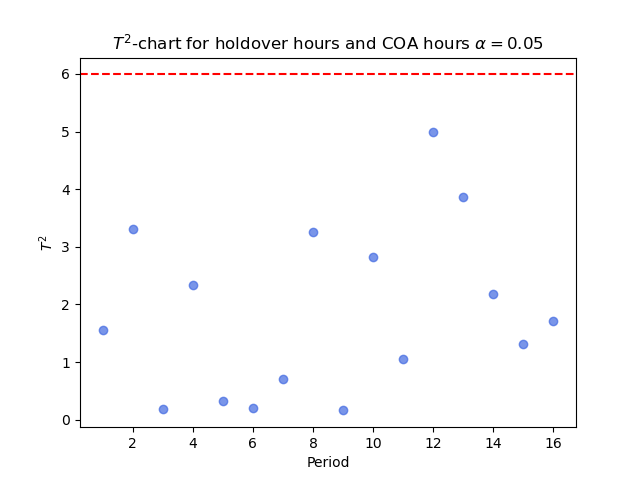
\includegraphics[scale=0.65]{./python/chapter-5/Question-5-25-T2.png}
\end{figure}

\begin{figure}[H]
    \centering
    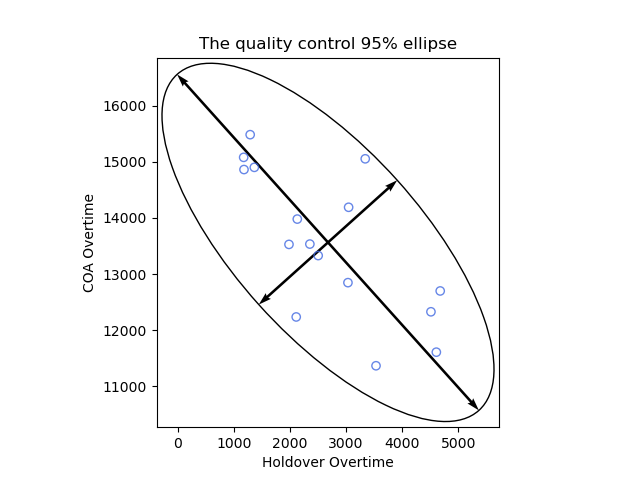
\includegraphics[scale=0.65]{./python/chapter-5/Question-5-25-QC-Ellipse.png}
\end{figure}


The $T^{2}$-chart shows all values less than the critical value $\chi_{2}^{2} = 5.99$, and the 95\% quality control ellipse shows all points within the ellipse. Because of this we would consider the process to be in control (stable). I would say these plots take the correlation into account. In the QC ellipse we can see that as holdover overtime increases, COA overtime decreases. We can also see that observation 12 has the highest $T^{2}$ value and is the observation closest to being outside the 95\% ellipse. However, all of the points are within the ellipse, so there's no need to construct individual $\bar{X}$ charts.